\section{Fitting \loglin\ models} \label{sec:loglin-fitting}

Fitting a \loglin\ model is a process of
deciding which association terms are significantly different from zero;
these terms are included in the model that is used to explain the
observed frequencies.  Terms which are excluded from the model go
into the residual or error term, which reflects the overall
badness-of-fit of the model.  The usual goal of \loglin\ modeling
is to find a small model (few association terms) which nonetheless achieves a
reasonable fit (small residuals).

\subsection{Goodness-of-fit tests} \label{sec:loglin-goodfit}

For an \nway\ table, goodness-of-fit tests for a \loglin\ model
attempt to answer the question ``How well does the model reproduce
the observed frequencies?''
To avoid multiple subscripts, let $\vec{n} = n_1, n_2, \ldots , n_N$ denote
the observed frequencies in a table with $N$ cells
with corresponding fitted frequencies
$\widehat{\vec{m}} = \widehat{m}_1, \widehat{m}_2, \ldots , \widehat{m}_N$
according to a particular \loglin\ model.
The standard goodness-of-fit statistics are sums over the cells
of measures of the difference between the $\vec{n}$ and $\widehat{\vec{m}}$.
The most commonly used are the familiar Pearson chi-square,
\begin{equation*}%\label{eq:pchi}
\chisq = \sum_i \frac{( n_i - \widehat{m}_i )^2}{\widehat{m}_i}
\comma
\end{equation*}
and the \LR\ \GSQ\ or deviance statistic,
\begin{equation}\label{eq:pgsq}
\GSQ =  2 \sum_i n_i \, \log ( n_i / \widehat{m}_i )
\period
\end{equation}
Both of these statistics have asymptotic \chisq\
distributions when all expected frequencies are large.%
\footnote{A wider class of test statistics including \chisq\
and \GSQ\ as special cases is
described by \citet{CressieRead:84} and \citet{ReadCressie:88}.
Except in bizarre or borderline
cases, all members of this class provide the same conclusions when 
expected frequencies are at least moderate (all $\widehat{m} > 5$).}
The (residual) degrees of freedom are the number of cells ($N$) minus the
number of estimated parameters.

In practice we often find that several models have an acceptable fit
or, sadly, that none do (usually because we are ``blessed'' with a
large sample size).
It is helpful to compare competing models statistically,
and two strategies are particularly useful in these cases.

The \LR\ \GSQ\ statistic is unique in that one can compare two
\glossterm{nested models} by their difference in \GSQ\ s,
which has a \chisq\ distribution on the difference in degrees of
freedom.
Two models, $M_1$ and $M_2$, are nested when one, say, $M_2$, is
a special case of the other.  That is, model $M_2$ (with $\nu_2$ residual df)
contains a subset of
the parameters of $M_1$ (with $\nu_1$ residual df),
the remaining ones being effectively set to zero.
Model $M_2$ is therefore more restrictive and cannot fit the data better
than the more general model $M_1$, i.e., $\GSQ (M_2) \ge \GSQ (M_2)$.
The least restrictive of all models, with $\GSQ = 0$ and $\nu=0$ df is
the saturated model for which $\widehat{\vec{m}} = \vec{n}$.

Assuming that the less restrictive model $M_1$ fits, the difference in
\GSQ,
\begin{eqnarray}
\Delta \GSQ \equiv \GSQ ( M_2 \given M_1 ) 
& = & \GSQ ( M_2 ) - \GSQ ( M_1 ) \label{eq:gsqnest1} \\
& = & 2 \sum_i n_i \, \log ( \widehat{m}_{i1} / \widehat{m}_{i2} ) \label{eq:gsqnest2}
\end{eqnarray}
has a chi-squared distribution with df = $\nu_2 - \nu_1$.
The last equality \eqref{eq:gsqnest2} follows from substituting in \eqref{eq:pgsq}.

Rearranging terms in \eqref{eq:gsqnest1}, we see that we can partition
the $\GSQ ( M_2 )$ into two terms,
\begin{equation*}
\GSQ ( M_2 ) = \GSQ ( M_1 ) + \GSQ ( M_2 \given M_1 )
\period
\end{equation*}
The first term measures the difference between the data and the more
general model $M_1$.  If this model fits, the second term measures the
additional lack of fit imposed by the more restrictive model. 
In addition to providing a more focused test, $\GSQ ( M_2 \given M_1 )$
also follows the chi-squared distribution more closely when some
$\{ m_i \}$ are small
\citep[\S 7.7.6]{Agresti:90}.

Alternatively, a second strategy uses other measures that combine
goodness-of-fit with model parsimony and may also be used to compare
non-nested models.  The statistics described below are all cast in
the form of badness-of-fit relative to degrees of freedom, so that
smaller values reflect ``better'' models.


The simplest idea \citep{Goodman:71}
is to use $\GSQ / df$
(or $\chisq / df$), which has an expected value of 1 for a good-fitting
model.  This type of measure is routinely
reported by \PROC{GENMOD}.

The \emph{Akaike Information Criterion} (AIC) statistic
\citep{Akaike:73} is a very general criterion for model selection
with maximum likelihood estimation, based on the idea of maximizing
the information provided by a fitted model.  AIC is defined generally
as 
\begin{equation*}
\mbox{AIC} = -2 \log \mathcal{L} + 2 k
\end{equation*}
where $\log \mathcal{L}$ is the maximized log likelihood and $k$ is
the number of parameters estimated in the model,
so better models correspond to \emph{smaller} AIC.  For \loglin\ models,
minimizing AIC is equivalent to minimizing
\begin{equation*}
\mbox{AIC}^{\star} = \GSQ - 2 \nu
\end{equation*}
where $\nu$ is the residual df.  This form is easier to calculate by hand
from the output of any procedure if AIC is not reported.
\citet[\S IV.8]{Christensen:97} shows that
AIC is a close analog of \citet{Mallows:73} $C_p$ statistic, commonly used
for model selection in regression.

A third statistic of this type is the BIC or \citet{Schwartz:78} criterion
\begin{equation*}
\mbox{BIC} = \GSQ -  \nu \,\log (n)
\end{equation*}
where $n$ is the total sample size.  Both AIC and BIC penalize the fit
statistic for increasing number of parameters.
BIC also penalizes the fit directly with sample size, and so expresses
a preference for less complex models than AIC as the sample size increases.
But the sample size is fixed for a given \mway\ table, so the argument
for BIC seems less clear for \loglin\ models.

Finally, some users are comforted to know that there are analogs 
in \loglin\ models of the
familiar $R^2$ and Adjusted $R^2$ often used to assess the goodness-of-fit
of regression and ANOVA models.
In these standard linear models, $R^2$ is defined as
\begin{equation*}
R^2 = 1 - \frac{SSE (M_1)}{SSE (M_0)} =
  \frac{SSE (M_0) - SSE (M_1)}{SSE (M_0)}
\end{equation*}
where $SSE (M_1)$ is the error sum of squares for a model of interest, and
$SSE (M_0)$ is the error sum of squares for the smallest null model,
usually the model with an intercept only.
Hence, $R^2$ gives the proportion of the variation of the data explained
by the model $M_1$, or equivalently, the proportion of error removed by
the model.

In \loglin\ models, the deviance \GSQ\ is analogous to the SSE in a
classical linear model, and so we may define
\begin{equation}\label{eq:rsq-llm}
R^2 = 1 - \frac{G^2 (M_1)}{G^2 (M_0)} =
  \frac{G^2 (M_0) - G^2 (M_1)}{G^2 (M_0)}
\end{equation}
For a \loglin\ model, it usually makes sense to take the null model $M_0$
as the smallest possible interesting model.
For example, in models with one or more response variables, $R_1 , \dots$,
and two or
more explanatory variables $E_1 , E_2, \dots$,
the null model is usually $[ E_1 E_2 \dots ] [R_1] \dots$,
including the highest-order interaction of the explanatory variables.

As in linear models, the $R^2$ defined in \eqref{eq:rsq-llm} can never
decrease as more parameters are fitted (so residual df, $\nu$, decrease)
An adjusted $R^2$, taking model complexity into account is defined
as
\begin{equation*}
 R^2 = 1 - \frac{G^2 (M_1) / \nu_1 }{G^2 (M_0) / \nu_0}
 \comma
\end{equation*}
which is the same adjustment used in regression models.
The largest value of the adjusted $R^2$ will occur for the model having
the smallest value of $\GSQ / \nu$.


\subsection{Software}
The SAS System offers a variety of facilities for fitting \loglin\
models.  \PROC{CATMOD}, a very
general procedure for categorical data modeling, provides a \stmt{LOGLIN}{CATMOD}
tailored for \loglin\ models.
\PROC{GENMOD} includes \loglin\ models as a special case of
generalized linear models, as a model for log frequency, with a
Poisson distribution for errors.
In \INSIGHT, the \textsf{Fit (Y X)} menu also
fits generalized linear models;  for a \loglin\ model,
you select Poisson as the response distribution and Log as the
link function on the \textsf{Method} panel.
Finally, \IML\ provides the \pname{IPF} function,
which fits a \loglin\ model by the method of iterative proportional fitting.

\subsection{Using \PROC{CATMOD}}
For \PROC{CATMOD}, all table variables are considered dependent
variables and are treated as discrete factors by default.
Thus,
for \loglin\ models, the \stmt{MODEL}{CATMOD}
should specify
all \ctab\ factors, in the form
\pname{A*B*C ... = }\verb|_RESPONSE_|.
The
\verb|_RESPONSE_| keyword indicates that
the cell frequencies in the \ctab\ formed by the variables
\pname{A, B, C, ...} are being modeled.
The
\stmt{LOGLIN}{CATMOD} is used
to specify the model to be fit.  When the data are in
frequency form, as is typical, you use a \stmt{WEIGHT}{CATMOD} to specify the
frequency variable giving the cell count.

\begin{Example}[berkeley5]{Berkeley admissions}
Data on admission to the six largest graduate departments at
Berkeley was examined graphically in \chref{ch:twoway}
and in \chref{ch:mosaic}.  The data are
contained in the \Dset\ \pname{berkeley}, listed in
\datref{dat:berkeley}.
The \loglin\ model \eqref{eq:berk1} can be fit to this data
with \PROC{CATMOD} as shown below.

\begin{listing}
proc catmod order=data data=berkeley;
   format dept dept. admit admit.;
   weight freq;
   model dept*gender*admit=_response_ /
         ml noiter noresponse nodesign noprofile pred=freq ;
   loglin admit|dept|gender @2 / title='Model (AD,AG,DG)';
 run;
\end{listing}
On the \stmt{LOGLIN}{CATMOD}, the ``bar'' notation (\pname{admit|dept|gender @2}) means all terms up to two-way associations.
The printed output includes the table of fit statistics shown in \outref{out:catberk5.1}, which indicates that only
the two-way terms \pname{DEPT*ADMIT} and \pname{DEPT*GENDER} are significant.  In
particular, there is no association between Gender and Admission,
controlling for Department.
Several models may be fit within one \PROC{CATMOD} step.
We drop the \pname{GENDER*ADMIT} term
in the following model, giving the model fit statistics in
\outref{out:catberk5.2}.

\begin{listing}
   loglin admit|dept dept|gender / title='Model (AD,DG)';
 run;
\end{listing}
which gives the fit statistics shown in \outref{out:catberk5.2}.

\begin{Output}[htb]
\caption{Berkeley admissions data: Model [AD] [AG] [DG], fit with \PROC{CATMOD}}\label{out:catberk5.1}
\small
\verbatiminput{ch7/out/catberk5.1}
\end{Output}

\begin{Output}[htb]
\caption{Berkeley admissions data: Model [AD] [DG], fit with \PROC{CATMOD}}\label{out:catberk5.2}
\small
\verbatiminput{ch7/out/catberk5.2}
\end{Output}

The fit of the model $[AD] [DG]$ is not much worse than that of the
model $[AD] [AG] [DG]$.
Nevertheless, neither model fits very well, as judged by the
\LR\ \GSQ\ statistics.
We will see why in the next Example.
\end{Example}


\subsection{Using \PROC{GENMOD}}
With \PROC{GENMOD} \loglin\ models are fit directly in the style of
Model \eqref{eq:berk1},
that is, as a model for the log frequency with a Poisson distribution.
Whereas \PROC{CATMOD} assumes that all factor variables are categorical
(unless declared as quantitative in a \stmt{DIRECT}{CATMOD}),
\PROC{GENMOD} follows the scheme of \PROC{GLM}, so variables are assumed
to be quantitative, unless declared categorical in a
\stmt{CLASS}{GENMOD}.


\begin{Example}[berkeley6]{Berkeley admissions}
The homogeneous association model $[AD] [GD] [AG]$, \eqref{eq:berk1}, may be fit as a generalized linear
model for log frequency with \PROC{GENMOD} as shown below, and produces the model fit
statistics shown in \outref{out:genberk2.1}.  The Deviance statistic is identical to
the \LR\ \GSQ\ shown in \outref{out:catberk5.1}.
The keywords \pname{type3 wald} give Type III Wald tests of individual terms,
similar to the maximum likelihood ANOVA table produced by \PROC{CATMOD}.
\begin{listing}
proc genmod data=berkeley;
   class dept gender admit;
   model freq = dept|gender|admit@2 / dist=poisson link=log type3 wald;
\end{listing}

\begin{Output}[htb]
\caption{Berkeley admissions data: Model [AD] [AG] [DG], fit with \PROC{GENMOD}}\label{out:genberk2.1}
\small
\verbatiminput{ch7/out/genberk2.1}
\end{Output}

We fit the model $[AD] [GD]$ as shown below.
This is the conditional independence model, $A \perp G \given D$.  Because this model does not
fit well, we obtain the residuals among the observation statistics
with the statement \pname{make 'obstats' out=obstats;}.
The factor variables \pname{dept gender admit} are merged with the \pname{obstats} \Dset,
translated to more meaningful labels, and
we request a mosaic display with the \macro{MOSAIC}.
\begin{listing}
proc genmod data=berkeley;
   class dept gender admit;
   model freq = admit|dept gender|dept / dist=poisson obstats residuals;
   make 'obstats' out=obstats;
data obstats;
   merge berkeley obstats;
   D = put(dept, dept.);
   if admit=1
      then A='Admitted';
      else A='Rejected';
   if gender='F'
      then G = 'Female';
      else G = 'Male';

%mosaic(data=obstats, var=A G D, vorder=A G D, count=freq,
   resid=streschi, cellfill=dev, split=H V,
   title=Model: [AdmitDept] [GenderDept]);
\end{listing}
The mosaic display, shown in \figref{fig:mosaic9a}, indicates that this model fits well
(residuals are small)
except in Department A.
%% one figure
\begin{figure}[htb]
  \centering
  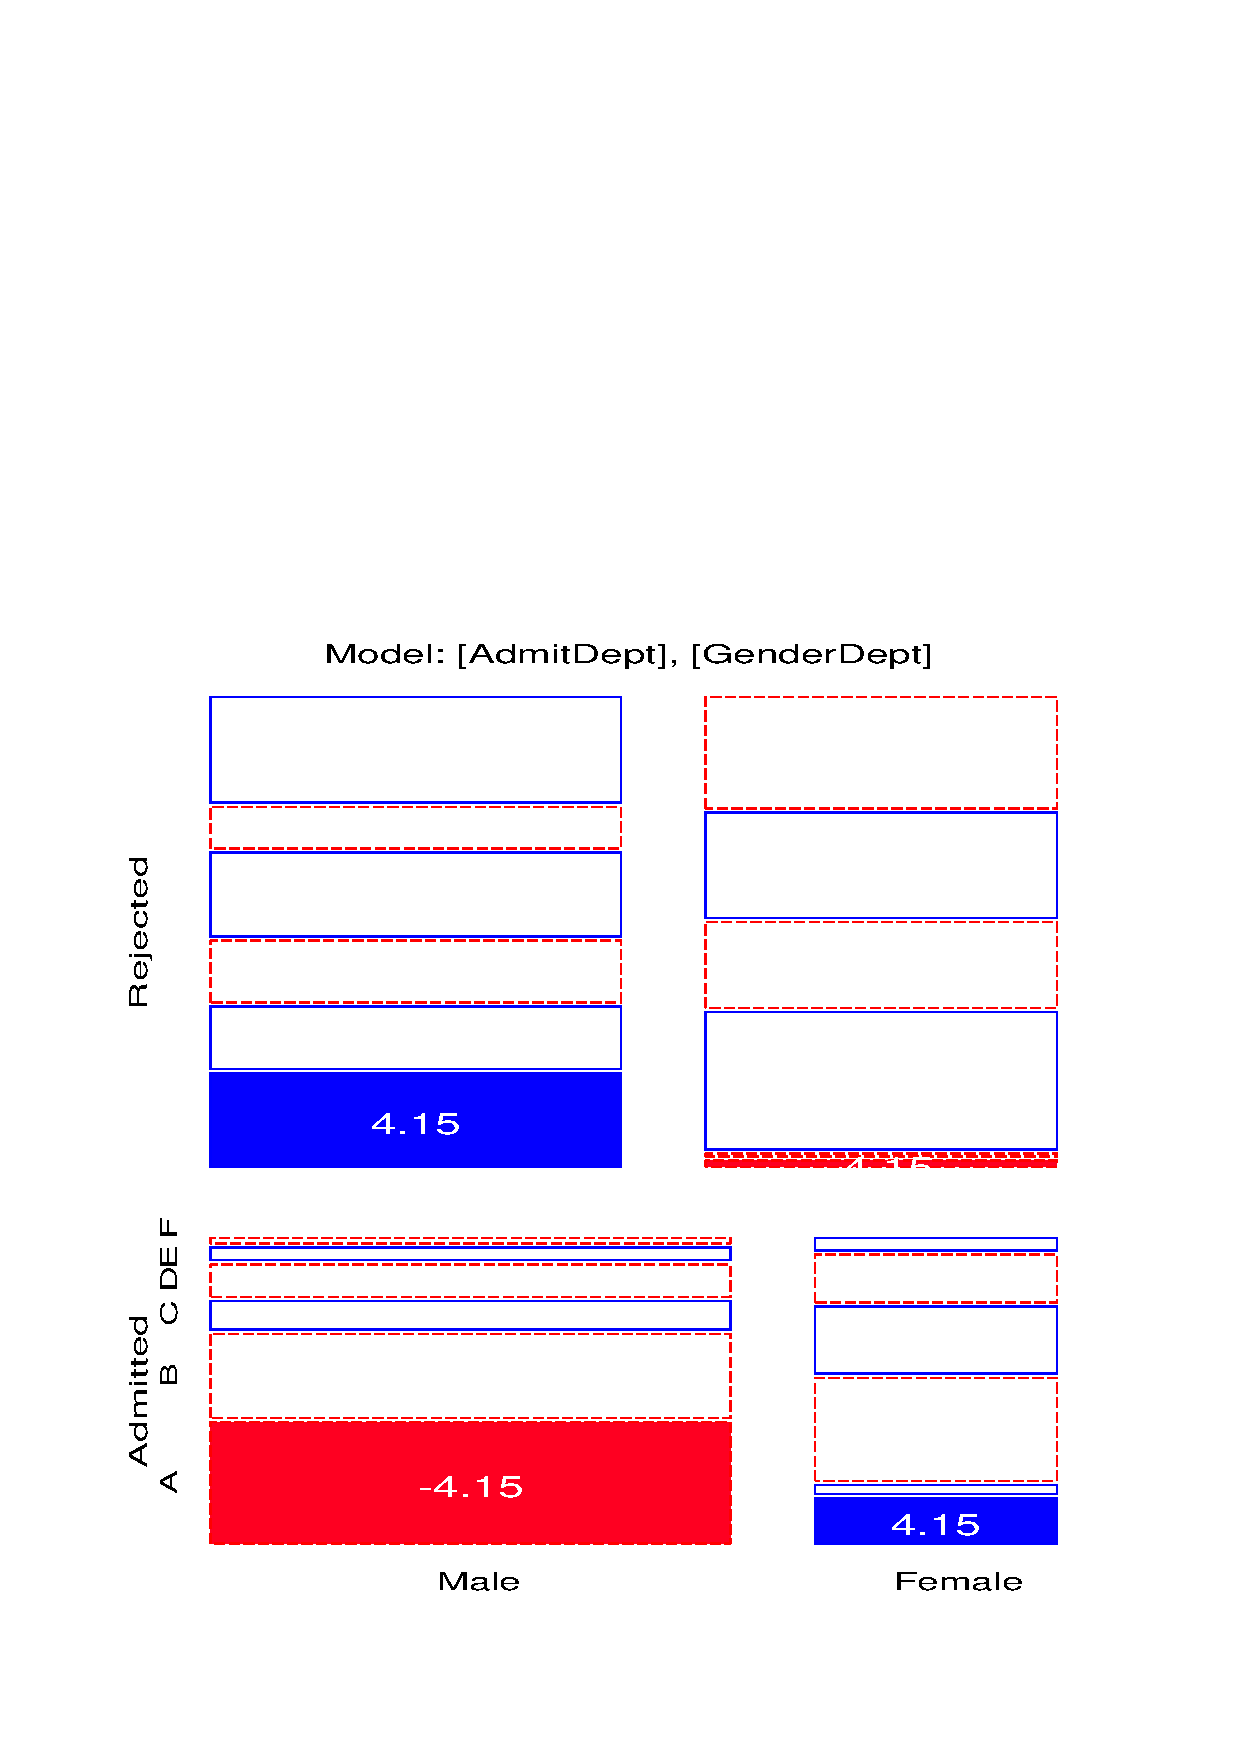
\includegraphics[scale=.6]{mosaic9a}
  \caption{Mosaic display for Berkeley admissions data}%
  \label{fig:mosaic9a}
\end{figure}
This suggests a model which allows an association between Admission and Gender in Department
A only,
\begin{equation}\label{eq:berk2}
  \log \,  m_{ijk}  =
  \mu
  +  \lambda_i^A
  +  \lambda_j^D
  +  \lambda_k^G
  +  \lambda_{ij}^{AD}
  +  \lambda_{jk}^{DG}
  +  \delta_{j=1} \lambda_{ik}^{AG} \comma
\end{equation}
where $\delta_{j=1}$ equals 1 for Department A ($j=1$) and is zero otherwise.
This model asserts that Admission and Gender are conditionally independent,
given Department, except in Department A.  It has one more parameter than
the conditional independence model, $[AD] [GD]$.
Model \eqref{eq:berk2} may be fit with \PROC{GENMOD} by constructing a variable
equal to the interaction of \pname{gender} and \pname{admit}
with a dummy variable having the value 1 for Department A and 0 for other departments.
\begin{listing}
data berkeley;
   set berkeley;
   dept1AG = (gender='F') * admit * (dept=1);

proc genmod data=berkeley;
   class dept gender admit;
   model freq = dept|gender dept|admit dept1AG / dist=poisson type3 wald;
\end{listing}
The model fit statistics and Type III tests for model \eqref{eq:berk2} are shown in
\outref{out:genberk2.2}.  This model fits very well indeed.
The parameter estimate, $\widehat{\lambda}_{ik}^{AG} = 1.052$ may be interpreted as
the log odds ratio of admission for females as compared to males in Dept. A.
The odds ratio is $\exp(1.052) = 2.86$, the same as the value calculated from the
raw data (see \secref{sec:twoway-fourstrat}).
\begin{Output}[htb]
\caption{Berkeley admissions data: Model \eqref{eq:berk2}, fit with \PROC{GENMOD}}\label{out:genberk2.2}
\small
\verbatiminput{ch7/out/genberk2.2}
\end{Output}
\end{Example}


\subsection{Using \INSIGHT}
\INSIGHT\ can be invoked either as a procedure (\PROC{INSIGHT})
or interactively from the Display Manager, through menus (\textsf{Globals}->\textsf{Analyze}->\textsf{Interactive data analysis}%
\footnote{In \sasver{7}, the menu choices are
\textsf{Solutions}->\textsf{Analysis}->\textsf{Interactive data analysis}})
or the command line (\textsf{insight}).
When you call \INSIGHT\ as a procedure, you can specify a \loglin\
model in a \stmt{FIT}{INSIGHT}, and obtain printed output from the
analysis.
When you invoke \INSIGHT\ interactively,
 \loglin\ models may be fit from the \textsf{Analyze}->
\textsf{Fit (Y X)} menu.
In either case, you must specify the response distribution to be Poisson,
and the Log link function.
In addition, \INSIGHT\ treats numeric variables as Interval (quantitative)
and character variables as Nominal by default.  For interactive use, you may
change the type of a numeric variable by clicking on the \textsf{Int} button
in the spreadsheet window.  For procedure use, you must create an
equivalent character variable first.

The following statements illustrate the use of \INSIGHT\ as a procedure,
fitting the model \eqref{eq:berk2}.  We first create character variables
\pname{A D G} with \Dstp\ statements.  
\INSIGHT\ does not understand ``bar'' notation, so the
model terms must be spelled out.

\begin{listing}
data berkeley;
   set berkeley;
   D = put(dept, dept.);
   if admit=1
      then A='Admitted';
      else A='Rejected';
   if gender='F'
      then G = 'Female';
      else G = 'Male';
   dept1AG = (gender='F') * admit * (dept=1);

%let _print_=on;
proc insight data=berkeley;
   fit freq = A D A*D G G*D dept1AG / resp=Poisson link=log label=cell;
   tables;
run;
\end{listing}
\INSIGHT\ offers far more opportunities for graphic output when used
interactively.  To fit a \loglin\ model, you must select
Poisson for the \textsf{Response Dist.} and Log for the
\textsf{Link Function} on the \textsf{Method} panel.
A variety of output statistics and residual plots are available from
the \textsf{Output} panel.

\figref{fig:berkeley2} shows a mosaic display for Admission and Department,
obtained from the menu choices \textsf{Analyze}->\textsf{Box Plot/Mosiac Plot (Y)},
which illustrates how the proportion of applicants admitted declines
across departments (the $[AD]$ term).
\figref{fig:berkeley3} shows a plot of raw residuals, ($n_{ijk} - \widehat{m}_{ijk}$) against fitted frequencies, and a normal QQ plot of these
residuals, with the largest absolute values identified interactively.
These residual plots  are consistent with an
adequate model.

%% one figure
\begin{figure}[htb]
  \centering
  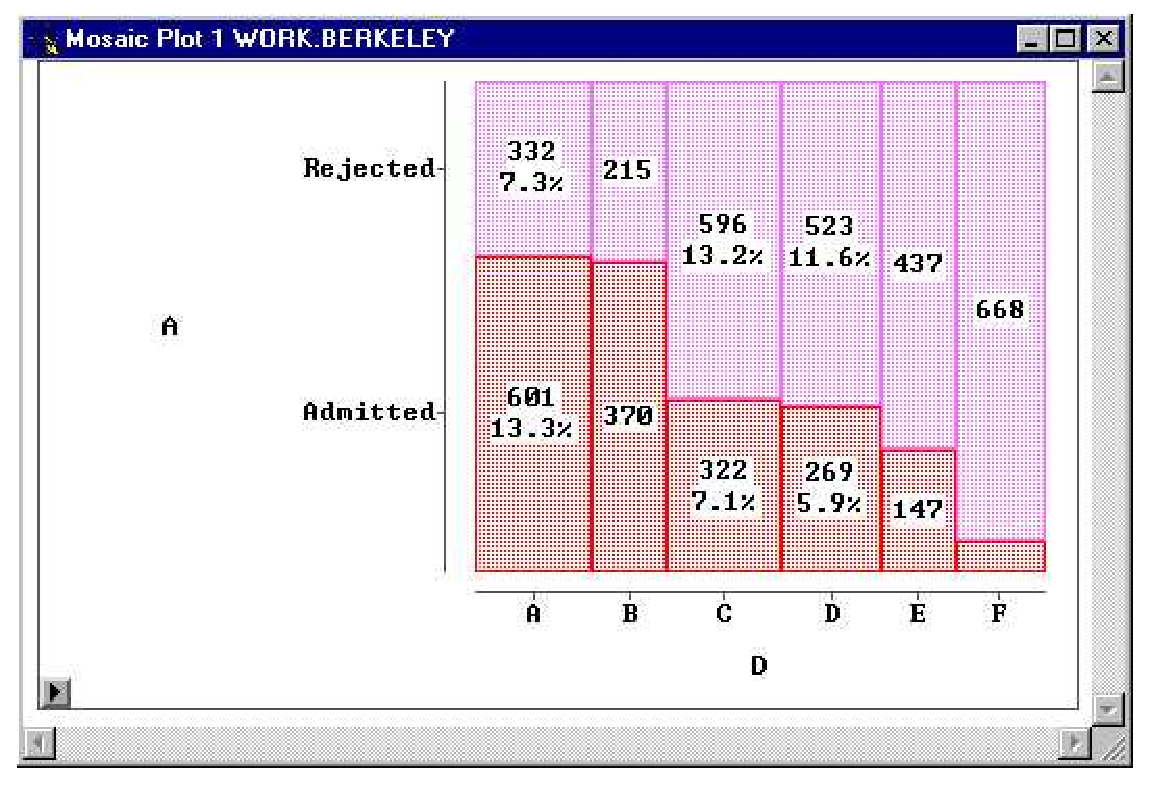
\includegraphics[scale=.6]{berkeley2}
  \caption{\INSIGHT\ mosaic display for Admission and Department}%
  \label{fig:berkeley2}
\end{figure}

%% one figure
\begin{figure}[htb]
  \centering
  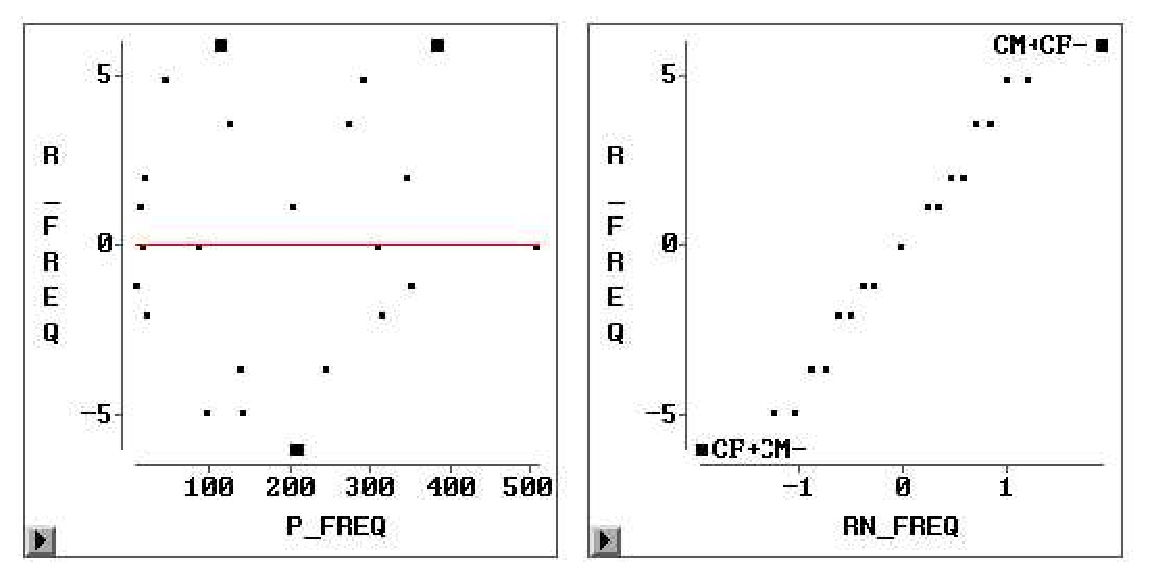
\includegraphics[scale=.6]{berkeley3}
  \caption{\INSIGHT\ residual plots for model \eqref{eq:berk2}}%
  \label{fig:berkeley3}
\end{figure}
